% !Mode:: "TeX:UTF-8"
% \textbf{计算专题------错误原因分析}

\begin{defproblem}{T16-A03-01}%
\begin{onlyproblem}%
化简:$ab\div \dfrac{a^2-1}{a+1}\cdot \dfrac{a-1}{ab^2}$,并选择你喜欢的整数$a$,$b$代入求值.

小刚计算这一题的过程如下:

\renewcommand{\arraystretch}{1.38}
$\begin{array}{r@{~}l@{\qquad\quad}l}
\text{解: 原式}&=ab\div \dfrac{(a+1)(a-1)}{a+1}\cdot \dfrac{a-1}{ab^2}&\text{①}\\
&=ab\times \dfrac{a+1}{(a+1)(a-1)}\cdot \dfrac{a-1}{ab^2}&\text{②}\\
&=\dfrac{1}{ab}&\text{③}
\end{array}$

当$a=1$,$b=1$时,原式=1.\hspace{7em}④

以上过程有两处错误,第一次出错在第{\_}{\_}{\_}{\_}{\_}{\_}{\_}步(填序号),原因:{\_}{\_}{\_}{\_}{\_}{\_}{\_}{\_}{\_}{\_}{\_}{\_}{\_}{\_}{\_}{\_};

还有第{\_}{\_}{\_}{\_}{\_}{\_}{\_}步出错(填序号),原因:{\_}{\_}{\_}{\_}{\_}{\_}{\_}{\_}{\_}{\_}{\_}{\_}{\_}{\_}{\_}{\_}{\_}{\_}{\_}{\_}.

请你写出此题的正确解答过程.
\end{onlyproblem}%
\begin{onlysolution}%
\begin{center}
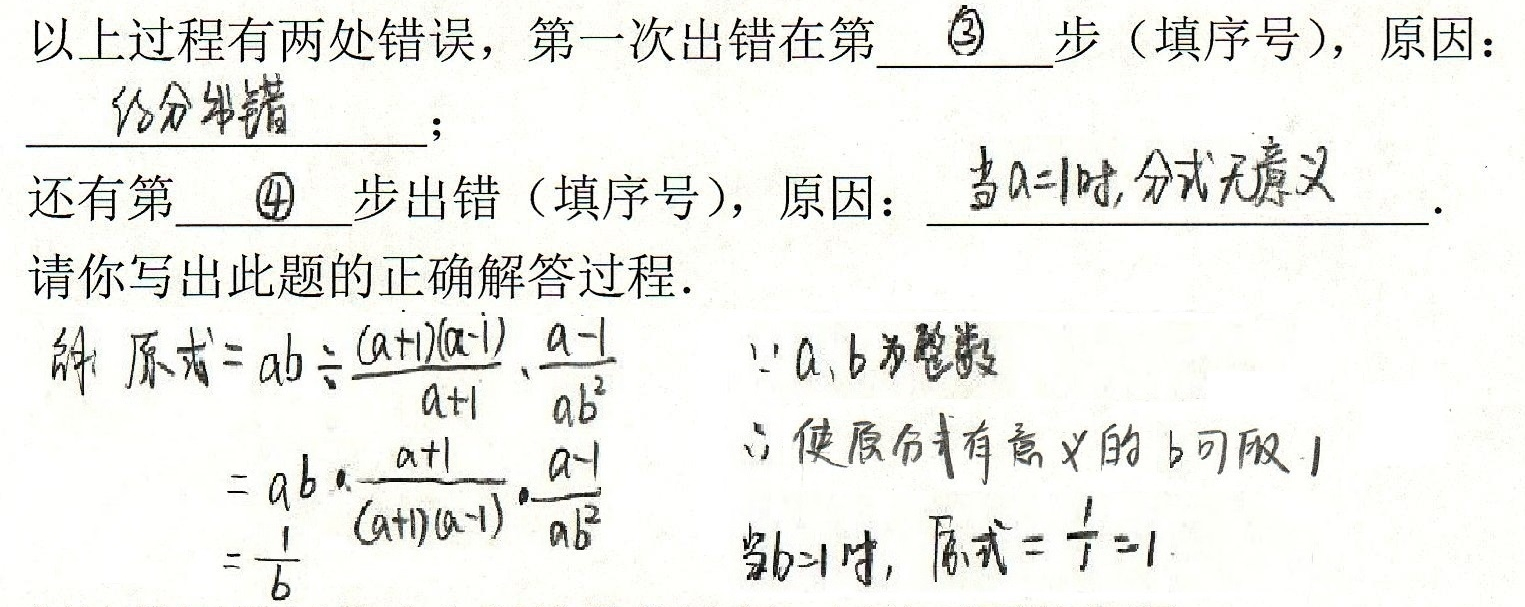
\includegraphics[width=.69\columnwidth]{T16-A03-01.jpg}
\end{center}
\end{onlysolution}%
\end{defproblem}


\begin{defproblem}{T16-A03-02}%
\begin{onlyproblem}%
阅读某同学解分式方程的具体过程,回答后面的问题.

解方程:$\dfrac{2}{x}+\dfrac{x}{x-3}=1$.

解:原方程可化为:

\noindent%
$\begin{array}{r@{~}l@{\qquad\quad}l}
 2(x-3)+x^2&=x(x-3)&\text{①}\\ 
 2x-6+x^2&=x^2-3x&\text{②}\\ 
 2x-3x+x^2-x^2&=6&\text{③}\\ 
 x&=-6&\text{④}
\end{array}$

检验:当$x=-6$时,各分母均不为0,

$x=-6$是原方程的解.\hspace{5em}⑤

请回答:(1)第①步变形的依据是{\_}{\_}{\_}{\_}{\_}{\_}{\_}{\_}{\_}{\_}{\_}{\_}{\_}{\_}{\_}{\_}{\_}{\_}{\_};

(2)从第{\_}{\_}{\_}{\_}步开始出现了错误,这一步错误的原因是{\_}{\_}{\_}{\_}{\_}{\_}{\_}{\_}{\_}{\_}{\_}{\_}{\_}{\_}{\_}{\_}{\_}{\_}{\_}{\_}{\_}{\_};

(3)请你写出此题的正确解答过程.

\end{onlyproblem}%
\begin{onlysolution}%
\begin{center}
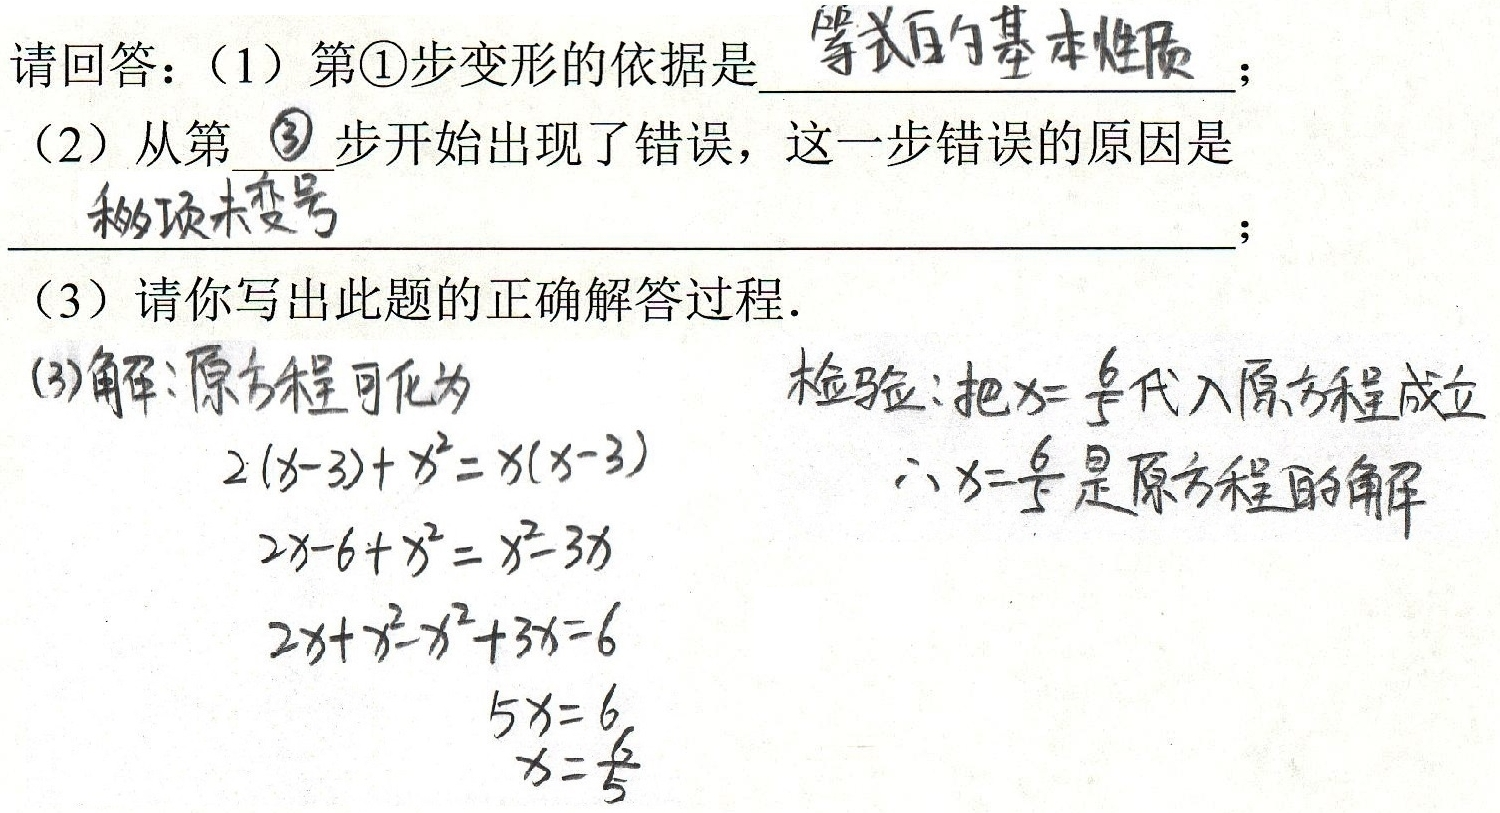
\includegraphics[scale=0.9]{T16-A03-02.jpg}
\end{center}
\end{onlysolution}%
\end{defproblem}


\begin{defproblem}{T16-A03-03}%
\begin{onlyproblem}%
解不等式组$\left\{\begin{array}{@{}lr}
-2x\le 6&\text{①}\\ 
4x\le 1+3x&\text{②}\\ 
\end{array}\right.$

请结合题意填空,完成本题的解答.

(1)解不等式①,得{\_}{\_}{\_}{\_}{\_}{\_}{\_}{\_}{\_}{\_}{\_}{\_}{\_}{\_},依据是:{\_}{\_}{\_}{\_}{\_}{\_}{\_}{\_}{\_}{\_}{\_}{\_}{\_}{\_}{\_}{\_}{\_}{\_}{\_}{\_}{\_};

(2)解不等式②,得{\_}{\_}{\_}{\_}{\_}{\_}{\_}{\_}{\_}{\_}{\_}{\_}{\_}{\_}{\_};

(3)把不等式①和②的解集在数轴上表示出来:
\vspace*{2\baselineskip}


(4)原不等式组的解集为{\_}{\_}{\_}{\_}{\_}{\_}{\_}{\_}{\_}{\_}{\_}{\_}.
\end{onlyproblem}%
\begin{onlysolution}%
\begin{center}
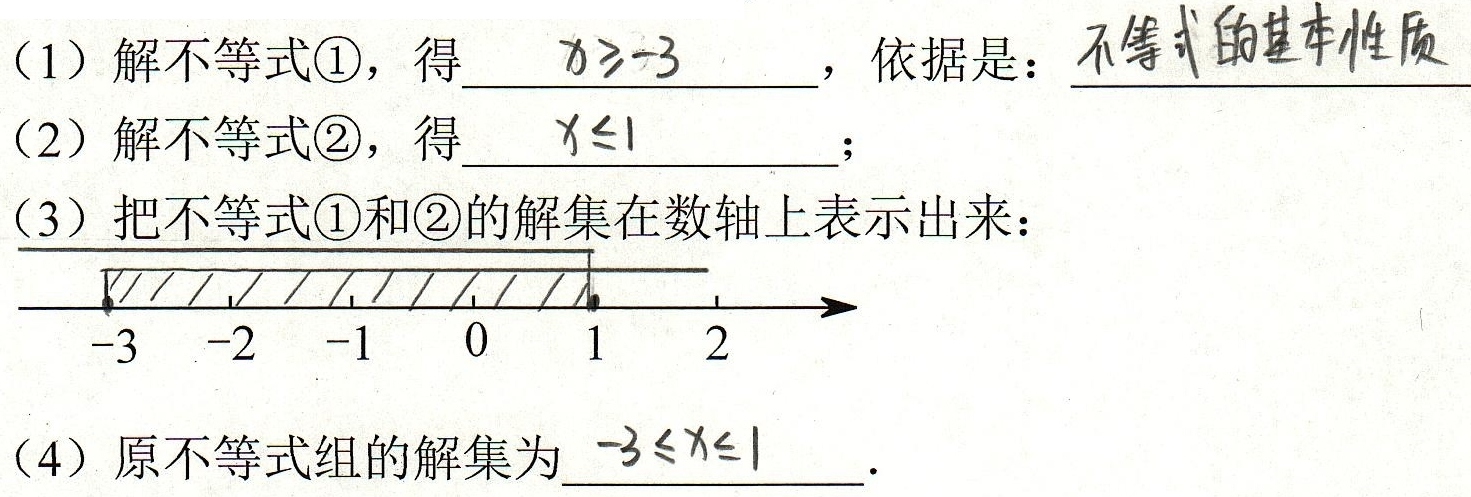
\includegraphics[scale=0.9]{T16-A03-03.jpg}
\end{center}
\end{onlysolution}%
\end{defproblem}


\begin{defproblem}{T16-A03-04}%
\begin{onlyproblem}%
某同学化简$a(a+2b)-(a+b)(a-b)$出现了错误,解答过程如下:
\begin{align*}
\text{原式}&=a^{2}+2ab-(a^{2}-b^{2})\tag*{(第一步)}\\
&=a^{2}+2ab-a^{2}-b^{2}\tag*{(第二步)}\\
&=2ab-b^{2}\tag*{(第三步)}
\end{align*}

(1)该同学解答过程从第{\_}{\_}{\_}{\_}{\_}步开始出错,错误原因是{\_}{\_}{\_}{\_}{\_}{\_}{\_}{\_}{\_}{\_}{\_}{\_}{\_}{\_};

(2)写出此题正确的解答过程.
\end{onlyproblem}%
\begin{onlysolution}%
\begin{center}
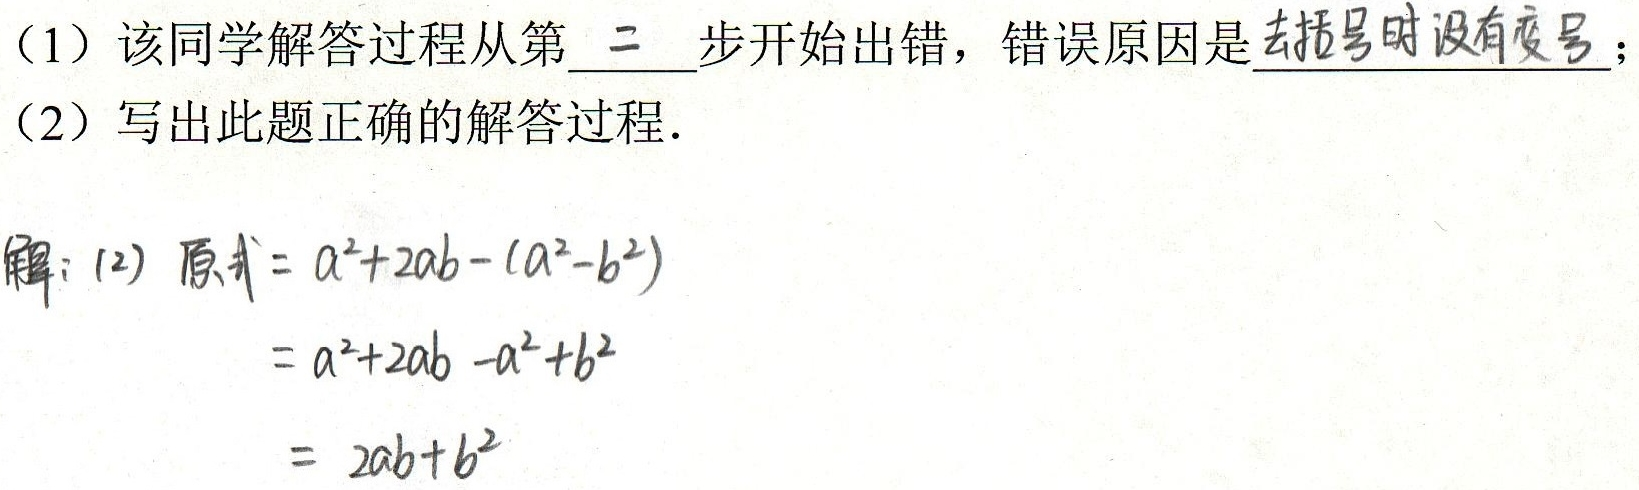
\includegraphics[width=.69\columnwidth]{T16-A03-04.jpg}
\end{center}
\end{onlysolution}%
\end{defproblem}


\begin{defproblem}{T16-A03-05}%
\begin{onlyproblem}%

课堂上,王老师出了这样一道题:

已知$x=2019-5\sqrt 3 $,求代数式$\dfrac{x^2-2x+1}{x^2-1}\div \left(1+\dfrac{x-3}{x+1}\right)$的值.

小明觉得直接代入计算太复杂了,同学小刚帮他解决了问题,并解释说:``结果与$x$无关''. 解答过程如下:
% \begin{align*}
% \text{原式}&=\dfrac{(x-1)^2}{(x+1)(x-1)}\div \dfrac{x+1+x-3}{x+1}\tag*{①}\\ 
% &=\dfrac{x-1}{x+1}\div \_\_\_\_\_\_\_\_\_\,\tag*{②}\\ 
% &=\dfrac{x-1}{x+1}\times \dfrac{x+1}{2(x-1)}\tag*{③}\\ 
% &=\dfrac{1}{2}\tag*{④}
% \end{align*}

\noindent%
$\begin{array}{r@{~}l@{\qquad\quad}l}
\text{原式}&=\dfrac{(x-1)^2}{(x+1)(x-1)}\div \dfrac{x+1+x-3}{x+1}&\text{①}\\ 
&=\dfrac{x-1}{x+1}\div \_\_\_\_\_\_\_\_\_\,&\text{②}\\ 
&=\dfrac{x-1}{x+1}\times \dfrac{x+1}{2(x-1)}&\text{③}\\ 
&=\dfrac{1}{2}&\text{④}
\end{array}$


当$x=2019-5\sqrt 3 $,原式$=\dfrac{1}{2}$.

(1)从原式到步骤①,用到的数学知识有:{\_}{\_}{\_}{\_}{\_}{\_}{\_}{\_}{\_}{\_}{\_}{\_}{\_};

(2)步骤②中的空白处的代数式为:{\_}{\_}{\_}{\_}{\_}{\_}{\_}{\_}{\_}{\_}{\_}{\_}{\_}{\_}{\_}{\_};

(3)从步骤③到步骤④,用到的数学知识有:{\_}{\_}{\_}{\_}{\_}{\_}{\_}{\_}{\_}{\_}{\_}{\_}{\_}{\_}{\_}.


\end{onlyproblem}%
\begin{onlysolution}%
\begin{center}
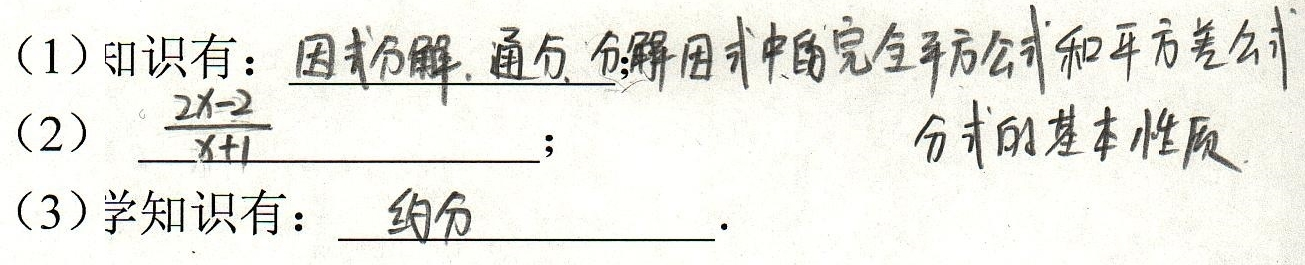
\includegraphics[width=.69\columnwidth]{T16-A03-05.jpg}
\end{center}
\end{onlysolution}%
\end{defproblem}


\begin{defproblem}{T16-A03-06}%
\begin{onlyproblem}%
某学生化简分式$\dfrac{1}{x+1}+\dfrac{2}{x^2-1}$出现了错误,解答过程如下:
\begin{align*}
\text{原式}&=\dfrac{1}{(x+1)(x-1)}+\dfrac{2}{(x+1)(x-1)}\tag*{第一步}\\ 
&=\dfrac{1+2}{(x+1)(x-1)}\tag*{第二步}\\ 
&=\dfrac{3}{x^2-1}\tag*{第三步} 
\end{align*}

(1)该学生解答过程是从第{\_}{\_}{\_}{\_}{\_}步开始出错的,其错误原因是{\_}{\_}{\_}{\_}{\_}{\_}{\_}{\_};

(2)请写出此题正确的解答过程.
\end{onlyproblem}%
\begin{onlysolution}%
\begin{center}
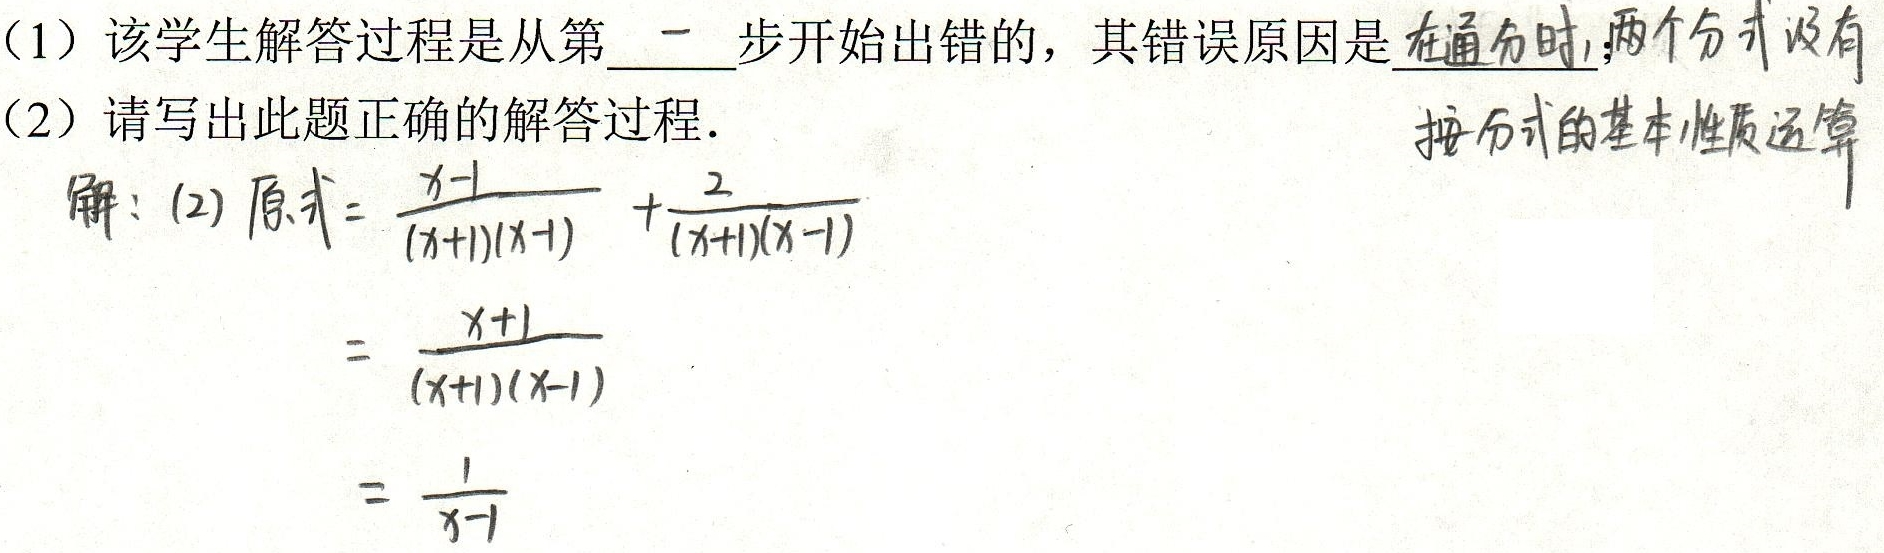
\includegraphics[scale=0.9]{T16-A03-06.jpg}
\end{center}
\end{onlysolution}%
\end{defproblem}

